\section{Pong}

In this section we describe application of Deep RL methods to a game of Pong implemented inside Unreal Engine 4 (UE4) environment.
Unreal Engine 4 is a suite of integrated tools for game developers to design and build games, simulations, and visualizations.

The main goals of this work is to prove that RL applied inside UE4 it's technically feasible solution: it's should be possible to efficiently train and apply model built with modern machine learning framework (in our case TensorFlow).

We achieve this by patching a plugin to support Python scripting inside UE4, implementing C++ module for capturing game screenshots, and creating TensorFlow-based Python controller for the player paddle.

\subsection{Environment}

We use physics based UE4 implementation of classical \href{https://en.wikipedia.org/wiki/Pong}{Pong} environment. 
\begin{figure}[h!]
\caption{Pong Screenshot}
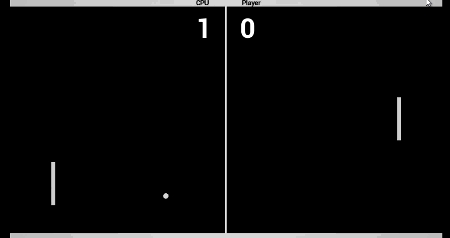
\includegraphics[width=\textwidth]{PongPhys}
\end{figure}

This screenshot from the environment shows main elements of the game:
\begin{enumerate}
    \item Paddles ---
        Every player controls a solid rectangle called paddle that can reflect the ball.
    \item Ball ---
        The ball is a rigid body that moves with a constant speed and reflects from the walls and paddles.
    \item Walls ---
        The walls are present on the top and on the bottom of the screen.
    \item Goals ---
        The left and right sides of the screen represent goals. In order to score a point, the player needs to hit the opposite goal with the ball.
    \item Scores ---
        The top part of the screen shows two numbers that are equal to the number of points each player have scored.
\end{enumerate}

The purpose of the game is to maximize the difference between your score and opponent score.

The human player uses raw pixels (screenshots) as an input during play, and outputs three types of actions using the keyboard:
\begin{itemize}
    \item Key up --- move paddle up
    \item Key down --- move paddle down
    \item Idle --- paddle stays at the same place
\end{itemize}

The game comes with the built-in AI controller that gets high-level features such as position and speed of the ball, position of his and opponent paddle as an input,
and uses rule-based approach to control the paddle.

\subsection{Python Scripting}

In Unreal Engine 4, the standard way to implement game logic is through writing C++ modules or using internal visual scripting language called Blueprints.
The C++ approach is more powerful and is used to implement core game logic and reusable modules, though in many cases it's overly verbose, and doesn't allow to quickly iterate on the solution due to slow compilation speeds.
On the other hand, blueprints are simple to create and understand, allow faster development cycles, yet not expressible enough in many cases.

When it comes to the modern machine learning engines, they are usually written in C++, while the public API that they provide comes in form of Python bindings.
While in principle it's possible to use TensorFlow C++ API, this approach limits the reuse of openly available RL algorithms implementations in Python, and slows down the research process due to the nature of the C++ language.

Due to all this reasons we looked into alternative languages support for UE4 and identified two candidates: Python and Lua.
Both languages are supported through third-party plugins available on GitHub, \href{https://github.com/facebook/UETorch}{UETorch} for Lua and \href{https://github.com/20tab/UnrealEnginePython}{UnrealEnginePython} for Python.

As the authors were more familiar with Python and TensorFlow, it was chosen as the primary language.
During this work, the original plugin was extended to support Python-based controllers in UE4.

The plugin allows users to write Python scripts that interact with UE4 engine by being able to access and mutate the internal state of the game.
This can be used to obtain current position of the ball and paddle, and giving the commands to move the paddle.

\subsection{RL Model}

We implement bot controller using TensorFlow machine learning framework \cite{tensorflow2015-whitepaper} to utilize GPU and multi-core CPU resources.
We use Deep Q-Network (DQN) \cite{mnih-dqn-2015} learning algorithm to train and control the bot.
The reward of +1 is given to the bot when it scores a point, and -1 when the opponent scores a point.

The bot is trained with fixed FPS 32. The screenshots are binarized and rescaled to resolution 80x80.

\subsection{Results}

We've built a Deep RL based controller that outperforms the standard rule-based bot, while using raw pixels as an input.
The training takes 6 hours on GPU and it takes 10 million iterations to beat the built-in scripted bot.

\begin{figure}[h!]
\caption{Average score difference over a set of 21 games.}
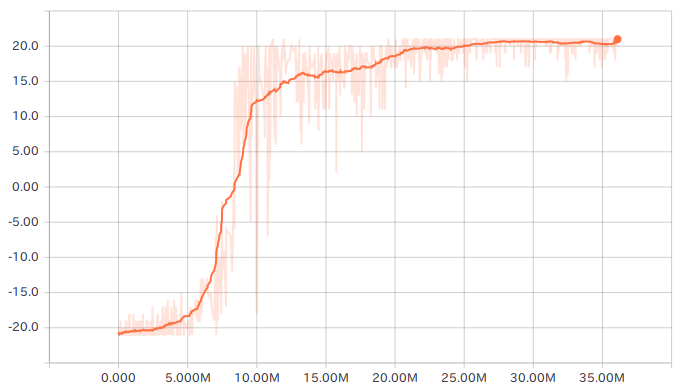
\includegraphics[width=\textwidth]{LearningCurve}
\end{figure}

The code implementation is available on \href{https://github.com/akashin/HSE_AI_Labs/tree/master/Lab_4}{GitHub}.